% Copyright (C) 2014 Miquel Sabaté Solà <mikisabate@gmail.com>
%
% This program is free software: you can redistribute it and/or modify
% it under the terms of the GNU General Public License as published by
% the Free Software Foundation, either version 3 of the License, or
% (at your option) any later version.
%
% This program is distributed in the hope that it will be useful,
% but WITHOUT ANY WARRANTY; without even the implied warranty of
% MERCHANTABILITY or FITNESS FOR A PARTICULAR PURPOSE.  See the
% GNU General Public License for more details.
%
% You should have received a copy of the GNU General Public License
% along with this program.  If not, see <http://www.gnu.org/licenses/>.

\documentclass[12pt,a4paper,twoside,openright]{book}

%%
% Packages

\usepackage[a4paper,width=150mm,top=25mm,bottom=25mm]{geometry}
\usepackage{indentfirst}
\usepackage{makeidx}
\usepackage[pdftex]{graphicx}
\usepackage{wrapfig}
\usepackage[utf8]{inputenc}
\usepackage[english]{babel}
\usepackage{url}
\usepackage{eurosym}
\usepackage{fancyhdr}


% Format of the chapter titles.
\usepackage{titlesec}
\titleformat{\chapter}
  {\normalfont\LARGE\bfseries}{\thechapter}{1em}{}
\titlespacing*{\chapter}{0pt}{3.5ex plus 1ex minus .2ex}{2.3ex plus .2ex}

% Header and footer.
\newcommand {\fncyfront}{%
\fancyhead[RO] {{\footnotesize \rightmark}}
\fancyfoot[RO] {\thepage}
\fancyhead[LE] {\footnotesize {\leftmark}}
\fancyfoot[LE] {\thepage}
\fancyhead[RE,LO]{}
\fancyfoot[C]{}
\renewcommand{\headrulewidth}{0.3 pt}}
\newcommand {\fncymain }{%
\fancyhead[RO]{{\footnotesize \rightmark}}
\fancyfoot[RO]{\thepage}
\fancyhead[LE]{{\footnotesize \leftmark}}
\fancyfoot[LE]{\thepage}
\fancyfoot[C]{}
\renewcommand {\headrulewidth}{0.3 pt}}

% Don't apply the fancy style on blank pages from the openright option.
\makeatletter
\def \cleardoublepage {\clearpage \if@twoside
\ifodd\c@page
\else\hbox{}\thispagestyle{empty}\newpage
\if@twocolumn \hbox {}\newpage \fi \fi \fi }
\makeatother


%%
% New commands.

% Add an extra vertical space.
\newcommand{\espai}{\par\vspace{5mm}}

% How I do lists.
\newcommand{\mylist}{

\begin{itemize}
\setlength{\itemsep}{1pt}
\setlength{\parskip}{0pt}
\setlength{\parsep}{0pt}}
\newcommand{\mylistend}{\end{itemize}}

% Needed for the title.
\newcommand{\HRule}{\rule{\linewidth}{0.5mm}}

% So the links in the Table of Contents actually work.
\usepackage{hyperref}
\hypersetup{
  colorlinks,
  citecolor=black,
  filecolor=black,
  linkcolor=black,
  urlcolor=black
}


%%
% Hey! Ho! Let's go!


\begin{document}


% The front matter is basically: the title, the ToC and the Preface.
\pagestyle{fancy}
\fncyfront
\frontmatter
% Copyright (C) 2014-2020 Miquel Sabaté Solà <mikisabate@gmail.com>
%
% This program is free software: you can redistribute it and/or modify
% it under the terms of the GNU General Public License as published by
% the Free Software Foundation, either version 3 of the License, or
% (at your option) any later version.
%
% This program is distributed in the hope that it will be useful,
% but WITHOUT ANY WARRANTY; without even the implied warranty of
% MERCHANTABILITY or FITNESS FOR A PARTICULAR PURPOSE.  See the
% GNU General Public License for more details.
%
% You should have received a copy of the GNU General Public License
% along with this program.  If not, see <http://www.gnu.org/licenses/>.


%%
% This file defines the title. It's created by hand by using the
% the instructions that were given in the following wiki page:
%       http://en.wikibooks.org/wiki/LaTeX/Title_Creation

\begin{titlepage}
\begin{center}

\textsc{\Large Barcelona School of Informatics}\\[0.5cm]

% Title
{ \small \HRule \\[0.4cm] }
{ \huge \bf Fita de seguiment \\[0.4cm] }
{ \small \HRule \\[0.4cm] }

% Author and supervisor
\begin{minipage}{0.4\textwidth}
\begin{flushleft} \large
\emph{Author:}\\
Miquel \textsc{Sabaté Solà}
\end{flushleft}
\end{minipage}
\begin{minipage}{0.4\textwidth}
\begin{flushright} \large
\emph{Director:} \\
Jordi \textsc{Garcia Almiñana}
\end{flushright}
\end{minipage}

\vfill

% Bottom of the page
{\large \today}

\end{center}
\end{titlepage}

\tableofcontents

\chapter{TODO: Preface}

Això serà un apartat {\bf molt} curt que bàsicament anirà de com està la
situació actual de la tecnologia, i com està afectant al desenvolupament de les
ciutats.

Ja et dic, una cosa exageradament curta (una pàgina màxima). Serveix per situar
al lector de la meva motivació personal per fer el projecte. També donaria els
típics agraïments.



\fncymain
\mainmatter

% All the elements of the project definition.

\section{TODO: The Project}

% We start by making a statement on the situation of the context.

\section{TODO: The Context}

Aquest és l'apartat on explicaré tot allò que envolta al projecte. Començaré
parlant del context d'aquesta plataforma (apartat 2.1): Quines tecnologies hi
ha, quin entorn estem vivint, etc.


% Then we talk about the problem we're trying to solve.

\subsection{TODO: The Problem}

Després de presentar el context, parlaré de quin problema intenta resoldre
aquest projecte (apartat 2.2).


% Proposal that fixes the stated problem.

\section{The Idea}

\subsection{Brief description}
\label{sec:description}

My Bachelor Degree Thesis consists on building a platform that addresses the
first problem described in section~\ref{sec:problem}. In particular, this
platform is able to:

\begin{enumerate}
  \itemsep0em
  \item Fetch and process data in realtime from any given city.
  \item Provide an easy way to extend it.
  \item Wrap the iCity platform, providing rich services instead of raw data.
\end{enumerate}

Thanks to the iCity platform, this platform is already able to respond to a
wide variety of data types. Some examples being:

\mylist
  \item Air pollution.
  \item Traffic.
  \item Irrigation control.
  \item Pedestrian flow.
\mylistend

At first I thought that I could also use data from the {\it
OpenDataBCN}\footnote{http://opendata.bcn.cat/opendata/en/} initiative.
However, I later discovered that this initiative only provides static content,
so I had to drop this idea.

Moreover, this platform has been designed to be as modular and agnostic as
possible. One of the consequences of this is that we could ideally integrate
more platforms (apart from the already existing iCity platform) without too much
trouble. This is not something that I have deeply researched, but it should be
doable.

\subsection{Wrapping the iCity Platform}

One of the main points of this project is that I am going to wrap the API of
the iCity Platform with endpoints of my own that will provide rich information
instead of raw data. This is really important because:

\begin{enumerate}
  \itemsep0em
  \item As a platform, we do not have to worry about the {\bf wide variety} of
data types, because the iCity platform is already abstracting away this issue.
  \item It gives more freedom to this {\bf platform}. As I pointed out in
section~\ref{sec:description}, this platform is not hardly tied to the iCity
platform. Therefore, even in the unlikely event that iCity gets deprecated or
dies, this platform can still fetch the data from somewhere else without too
much trouble. Of course, this other platform has to have the same guarantees as
iCity. On the other hand, if iCity is up and running, we could even consider
adding more sources of data to this platform without too much trouble.
  \item It gives the {\bf end developer} more freedom. This platform does not
replace iCity in any way. Therefore, developers can target the iCity platform
and this platform at the same time if they really want to. However, using this
platform should be enough.
  \item It is {\bf reliable}. The iCity platform is backed by the \ac{EU}. This
means that we can feel safe when using this platform.
\end{enumerate}

\subsection{Realtime}

This is the core concept behind this project. The real deal here is that all
the fetched data has to be processed in realtime. This requirement comes from
the way that the majority of targeted sensors work. Let's consider that we want
to track the levels of pollution of the air of our city. The levels of
pollution might vary during the day, and we might want to study how are these
variations occurring and how can we decrease the levels of air pollution from
this observation. Therefore, for this case we need to be tracking the levels of
pollution through the entire day. In this simple case, we realize that
processing this data in realtime is the only reliable solution to this.

In order to address this major neeed I have chosen the Storm framework. This
framework is the very base of this platform and it is thanks to this framework
that this platform can be even considered in the first place. I do not
want to get into many details in this section, but if you want to read more
about why I chose Storm, you might want to read the section~\ref{sec:state} of
this memoir.


% Showing some similar projects.

\subsection{TODO: Similar projects}

Després parlaré de coses com projectes similars (apartat 2.4) que existeixen,
alternatives, etc.


% Finally, talk about the challenges that I've been through while developing
% this project.

\section{TODO: Challenges and limitations}

També parlaré dels reptes que m'he trobat creant aquesta aplicació (apartat
2.5).


% An overview.

\chapter{An overview of the Platform}
\label{sec:overview}

% The big picture.
 
\section{The Big Picture}

\begin{figure}
  \centering
  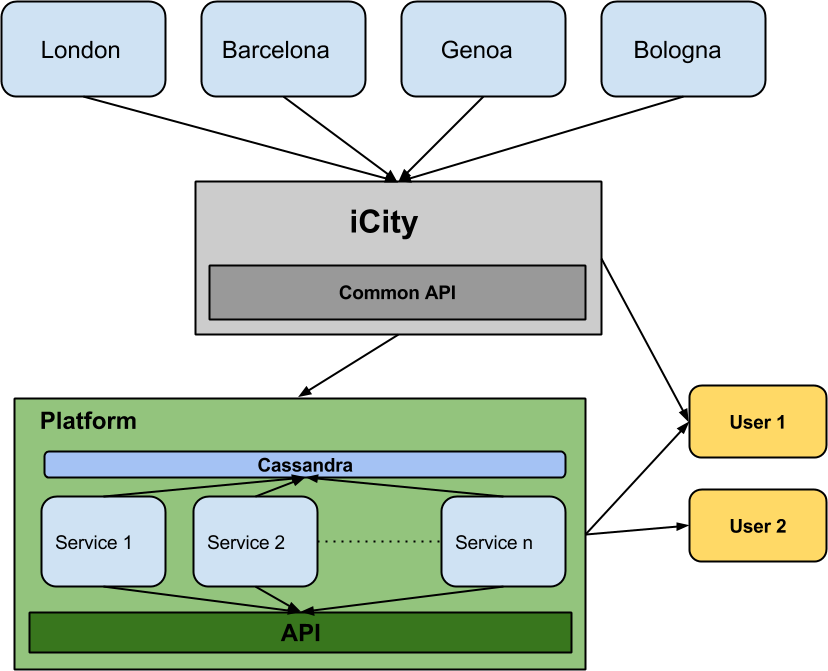
\includegraphics[scale=0.5]{overview/images/big.png}
  \caption{The architecture of the platform}\label{fig:architecture}
\end{figure}

In this section I am going to explain the architecture of the platform. It does
not enter into many details, but it is helpful in order to get a quick overview
on the design of the platform.

\begin{enumerate}
  \item The cities of London, Barcelona, Genoa and Bologna are {\bf producers}.
This list of cities will expand over time. Users are {\bf consumers}. They can
consume from either the iCity \ac{API}, from the \ac{API} from my platform, or
from both.
  \item The {\bf iCity} platform offers a common \ac{API} that integrates all
the cities. It gets the data from the different cities and allows the access of
this data to any user registered in the iCity platform.
  \item My {\bf platform} acts as a user of the iCity \ac{API} and users can
access the processed data.
  \item This platform is formed by {\bf several} services. These services
consume the data from the iCity platform in order to produce the requested
information.
  \item All the services from this platform are available through an {\bf
\ac{API}}.
  \item All the services are part of a {\bf Storm} topology.
  \item All the services share the {\bf state} of the platform, and it is stored
in a Cassandra instance.
\end{enumerate}



% Detailing the current start of the art.

\subsection{TODO: State of the Art}

Aquesta serà la secció més ``dura'' del projecte. Tractarè dels detalls més
tècnics del projecte. Començaré parlant de ``L'estat de l'art'' (apartat 3.1),
que va de com està la tecnologia actualment al voltant del projecte.


% The technologies being used.
 
\section{Used Technologies}

\subsection{Linux}

This platform targets Linux\footnote{http://www.linux.com/}. It is the Operating
System that I have used to develop this platform and the target of this
platform. This is because, for a variety of reasons, the vast majority of
Internet servers use Linux as their Operating system. Therefore, it makes
perfect sense to use Linux as the target operating system.

Note that this platform should also work in MacOS X and other \acs{BSD}
variants. However, I have not tested this platform in these operating systems,
so I cannot claim anything in regards to availability here.

\subsection{Java \& Scala}

Storm is implemented with Java and Clojure\footnote{http://clojure.org/}. This
two languages sit in top of
the \ac{JVM}. The \ac{JVM} is a virtual machine that can be used by any language
that knows how to produce bytecode for it. This includes languages such as:
Java, Clojure, Scala, Groovy, etc.

Moreover, all the languages on top of the \ac{JVM} can share packages. That is,
a \acs{JAR} file can be used as a library from any of these languages,
regardless of the language that was used in the library inside the \acs{JAR}
file. This means that languages like Scala can re-use the huge list of Java
packages that the community has implemented.

This means that in order to implement this platform I could have used any
language that sits on top of the \ac{JVM} without any real problem. I have
chosen Scala\cite{scala} because:

\mylist
  \item It is as {\bf fast} as Java, so there is no performance penalties
because of the language if we compare it with Java.
  \item It is {\bf modern}. Scala is a more recent language. This means that it
has had the influence of languages that are more recent than Java. This results
in Scala having many concepts from functional programming languages, concepts
from Python, Ruby, etc. It is an absolute pleasure to write Scala code.
  \item It has a {\bf robust} approach of concurrency. It is far more intuitive
than Java's lock/unlock mechanisms.
  \item It is {\bf stable}. Even if it is more recent than Java, Scala is rock
solid. As an example, big companies like Twitter and Foursquare have lots of
Scala code running on production.
\mylistend

\subsection{Storm}

As I have said in the section \ref{sec:state_storm}, the technology that I am
using to process all the data is Storm.

\subsection{Cassandra}
\label{sec:cassandra}

I do not store a lot of data in this platform, but I do store some data like
the state of the cluster. To achieve this I use Apache
Cassandra\cite{cassandra}. We could have chosen any \ac{DBMS} here to do the
job, but I have chosen Cassandra for the following reasons:

\mylist
  \item It has support for MapReduce. This is the main reason that I have
chosen Cassandra instead any other traditional \ac{DBMS} like PostgreSQL.
  \item It is {\bf fault-tolerant}, and supports several replication policies
across multiple clusters.
  \item It is {\bf descentralized}. There is no single point of failure.
  \item Its NoSQL nature has been helpful throughout the development of this
platform. Moreover, its query language (CQL) is quite similar to standard SQL,
so there has not been any major learning curve for me to use Cassandra.
\mylistend

One could argue that we do not need any \ac{DBMS} at all: we could just write
into temporary files or something like that. Even though would have simplified
things, this is not possible for the following reasons:

\begin{enumerate}
  \itemsep0em
  \item This platform can run in a multi-node cluster. Therefore, we would have
to pick a node among the others to store these temporary files. Doing this is,
of course, undesirable.
  \item Even if we pick a node from the cluster to keep these files: what if
this node melts down ? We cannot risk the integrity of the entire cluster to a
node that stores temporary files.
  \item CQL is a nice SQL-like language that gives us more flexibility doing
some operations on files.
\end{enumerate}

\subsection{Go}
\label{sec:go}

Go\footnote{http://golang.org/} is a programming language that emphasizes
concurrent programming. It was first developed by Google but it is now a truly
open source project. I use Go in the API layer. I have chosen Go for the
following reasons:

\begin{enumerate}
  \item Go puts special emphasis on {\bf concurrency}. Concurrency is also a
big deal in the Storm application. Therefore, it is a perfect match to use a
language that deals with concurrency and parallelism in an elegant and powerful
way.
  \item Go is a {\bf compiled} language. Therefore it is fast.
  \item It is {\bf simple}. As you can see in the language
reference\footnote{http://golang.org/ref/spec}, this language is pragmatic and
simple. Plus, programmers comming from languages like C and C++ will find a lot
of similarities with this language.
  \item It is {\bf stable}. Even if it is a fairly recent language, it is rock
solid. For example, companies like Google, Youtube, Dropbox, Soundcloud, etc.
are already using Go in production.
  \item The {\bf net/http} package is simple but really powerful. It abstracts
away a lot of problems regarding HTTP requests and responses.
\end{enumerate}



% The implementation of the project (a.k.a. the real deal).
 
\chapter{Implementation of the Platform}
\label{sec:implementation}

% Copyright (C) 2014-2015 Miquel Sabaté Solà <mikisabate@gmail.com>
%
% This program is free software: you can redistribute it and/or modify
% it under the terms of the GNU General Public License as published by
% the Free Software Foundation, either version 3 of the License, or
% (at your option) any later version.
%
% This program is distributed in the hope that it will be useful,
% but WITHOUT ANY WARRANTY; without even the implied warranty of
% MERCHANTABILITY or FITNESS FOR A PARTICULAR PURPOSE.  See the
% GNU General Public License for more details.
%
% You should have received a copy of the GNU General Public License
% along with this program.  If not, see <http://www.gnu.org/licenses/>.

\section{Introduction}

\subsection{Context}

This is the final report of the GEP course. The GEP course is part of my
Bachelor Degree Thesis, and consists of a set of deliveries and instructions
that has helped me in the preparation of my Thesis.

My Bachelor Degree Thesis is being presented at the Barcelona School of
Informatics and is directed by Mr. Jordi García Almiñana. The project was
originally envisioned by the director, and the author must develop a solution
for the given problem.

\subsection{Brief project description}

My Bachelor's Degree Thesis is about building an infrastructure that is
capable of providing a set of services from the data that has been collected
and processed. This data will come from initiatives like OpenData BCN and
iCity. This infrastructure will fetch and process all this data in realtime,
by using a set of new technologies that allow us to do so.

\subsection{Brief state of the art}

Since the appearence of the MapReduce algorithm, a lot of different
technologies have evolved so we can now fetch and process huge amounts of data.
This is important for the computer industry, but also for governments and other
associations.

We have a huge list of technologies that deal with Big data, but maybe the more
important ones are Hadoop and Storm. Storm is the base technology that I will be
using in this project. It's a modern and mature framework that will allow me to
build a realtime pipeline that is capable of fetching and processing huge
amounts of data.

\subsection{Purpose}

The purpose of this project is to provide a base infrastructure capable of
fetching and processing large amounts of data from iniciatives like OpenData
BCN and iCity to provide a set of services improving the actual situation.

 
\section{The core infrastructure}
\label{sec:implementation_core}

In this section and in the following sections \ref{sec:implementation_aqs} and
\ref{sec:implementation_bsp}, I will be talking about the Storm application.
I have named the Storm application ``Snacker''. That is why all the packages
name start by ``snacker''.

\subsubsection*{SBT}

The Storm application is built with the SBT\footnote{http://www.scala-sbt.org/}
toolchain. This toolchain is the {\it de facto} standard for Scala software and
it is similar to Java's Maven or Ant. The configuration for SBT resides inside
the project/Build.scala file. This file does the following:

\begin{enumerate}
  \itemsep0em
  \item It sets up basic information about this project.
  \item It tells SBT which version of Scala has to be used.
  \item It defines the different modules of this application.
  \item It tells SBT the dependencies for each module.
\end{enumerate}

SBT is the best toolchain that I have found to build Scala projects, and this
choice has affected on how the code is structured.

\subsubsection*{The main function and the core package}

The core infrastructure is divided into two Scala packages:

\begin{enumerate}
  \itemsep0em
  \item The package {\bf com.mssola.snacker}. This package contains the main
function and it is located in the ``src'' directory. This main function is
responsible for:
    \mylist
      \item Initializing the application.
      \item Loading the services.
      \item Executing the services.
    \mylistend
  \item The package {\bf com.mssola.snacker.core}. This package contains a set
of classes, objects and traits that will be used by the services. It is
located in the ``snacker-core'' directory. We can think of this package as the
main {\it library} for the services that are built on top of Storm.
\end{enumerate}

The most important thing about the com.mssola.snacker.core package is the {\bf
BaseComponent} object. This object is expected to be subclassed by each of the
services to be loaded. It is important because this object is responsible for
initializing each service and setting it up.


 
\section{Air Quality Sensors}
\label{sec:implementation_aqs}

\subsubsection*{London}

London is one of the cities that are available in the iCity platform. The city
of London has three services integrated in iCity:

\begin{enumerate}
  \itemsep0em
  \item {\bf Air Quality Sensors}. This service has sensors deployed all across
the city of London. These sensors mesure the air quality of the city. More
specifically, these sensors send data about the levels of: $NO_2$, SO, $O_3$,
PM10 and PM25.
  \item {\bf TFL Journey Planner}. This service gives access to developers to
the TFL API.
  \item {\bf Alert ME}. This platform is a Smart Home platform.
\end{enumerate}

The second and the third points are not really interesting in our case because
we need a source that is public and that sends data constantly. Therefore, for
this project I have picked the Air Quality Sensors platform.

\subsubsection*{Design and implementation}

Even if the Air Quality Sensors platform (AQS from now on) is the most complete
service from London, it has some major drawbacks:

\mylist
  \item The {\bf update rate} is low. Apparently the sensors from this platform
send data every hour. Nothing more, nothing less. This is quite frankly, a
poor update rate.
  \item There are lots of sensors that are not working. I have found that a lot
of the deployed sensors are not working at all.
\mylistend

Because of my points above, I have decided that I will not provide a streaming
API around this platform. Instead, I have built a minimal API around this
platform that only wraps up the API to provide some extra information.

The Storm application implements support for this platform through the {\bf
com.mssola.snacker.aqs} Scala package. This package is located in the
``snacker-aqs'' directory. The topology of this package is the following:

\begin{center}
  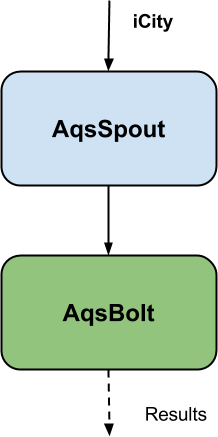
\includegraphics[scale=0.6]{implementation/images/aqs.png}
\end{center}

\begin{itemize}
  \itemsep0em
  \item The {\bf AqsSpout} is the only spout for this platform. This spout
fetches the data from iCity. After fetching it, this spout cleans and sends the
data to the AqsBolt.
  \item The {\bf AqsBolt} is the only bolt for this platform. This bolt
receives the data from the AqsSpout. After this, it performs some computations
and sends the results through a socket.
\end{itemize}

As I have previously said, this platform will not have a streaming API. This
means that when the API layer gets the data from the socket, it will close this
socket instantly. Therefore, the lifecycle of an HTTP request follows these
steps:

\begin{enumerate}
  \itemsep0em
  \item The API layer receives an HTTP request that points to the AQS service.
  \item The API layer subscribes to the AQS service for this request.
  \item The AQS module computes the results and sends them through the socket.
  \item The API layer receives the data and unsubscribes this request from AQS.
  \item The API layer generates a response with the given data.
\end{enumerate}

\subsubsection*{API endpoints}

The API for this service is minimal: I have implemented only one endpoint. This
is because the AQS service is really simple, and there are not a lot of
options here. This is the endpoint for this service:

\begin{center}
  /aqs/\{id\}/interval
\end{center}

The {\bf id} parameter has two possible values: ``all'' or a device id. The
possibility of getting the value for all the devices in a single request is
huge step forward in comparison of the iCity API. Besides the ``id'' parameter,
the developer has to include the following parameters in the request:

\mylist
  \item The {\bf from} and the {\bf to} parameters. These parameters are UNIX
timestapmps containing the interval of time.
  \item The {\bf property} parameter. Possible values are: ``no2'', ``so'',
``o3'', ``pm10'' and ``pm25''.
\mylistend

Calling this endpoint will result in a JSON response containing the values for
the specified properties and devices.

 
\section{Barcelona Sensors Platform}
\label{sec:implementation_bsp}

\subsubsection*{Barcelona}

Barcelona is one of the cities that are available in the iCity platform. The
city of Barcelona has invested heavily in the Smart Cities trend. Barcelona has
opened a lot of static data in the OpenDataBCN initiative. Apart from that,
Barcelona has three platforms integrated with the iCity platform:

\begin{enumerate}
  \itemsep0em
  \item The {\bf \ac{BSP}}. This platform allows any developer
to access the data sent by sensors that are distributed around the city. This
platform includes these kind of sensors:
    \mylist
      \item Environmental sensors (temperature, $NO_2$, $CO_2$, noise, etc.).
      \item Sustainability (level of capacity of the container waste).
      \item Traffic management (parking sensors).
      \item Walkers flows (number of pedestrian).
      \item Irrigation control (ground humidity, wind rain, temperature).
    \mylistend
  \item {\bf Smartcitizen Platform}. Smart Citizen is a platform to generate
participatory processes of people in the cities.
  \item {\bf IRIS}: the complaints and suggestions system.
\end{enumerate}

From these three possibilities I have picked the \ac{BSP}. This is because the
Smartcitizen platform is in an experimental stage and the IRIS platform is too
different to the London endpoint.

\subsubsection*{Storm}

The Storm application implements the support for \ac{BSP} in the Scala package:
{\bf com.mssola.snacker.bsp}. This package resides inside the ``snacker-bsp''
directory.

My original design consisted of one spout and five bolts (one for each kind of
sensor). However, I later decided that this was not realistic for the following
reasons:

\begin{enumerate}
  \itemsep0em
  \item The iCity \ac{API} does not make a distinction between the type of data.
Therefore, since there is not a real distinction, the data has to be treated
equally, regardless of the type.
  \item Conceptually, multiple bolts means that we are doing completely
different things with the same raw data. For example, with the same data one
bolt could store something on the database, and another bolt could compute
something else. This is not the case.
\end{enumerate}

Thus, the final design is fairly similar to the design of the London AQS
service:

\begin{figure}
  \centering
  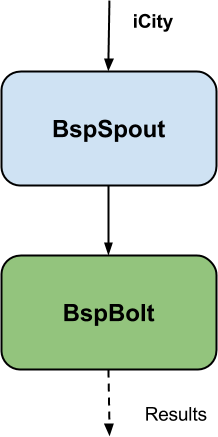
\includegraphics[scale=0.6]{implementation/images/bsp.png}
  \caption{BSP Topology}\label{fig:bsp_topology}
\end{figure}

\begin{enumerate}
  \itemsep0em
  \item The {\bf BspSpout} fetches the raw data from the iCity platform. After
this, it cleans up the data and sends it to the BspBolt.
  \item The {\bf BspBolt} receives the data from the BspSpout and performs a
set of computations. After this, it sends the results to the given socket.
\end{enumerate}

\subsubsection*{Streaming \ac{API}}

The update rate of the sensors from the \ac{BSP} is not very high, but at least
it is better than London. This is why I have decided that \ac{BSP} will have a
streaming \ac{API}. A streaming \ac{API} means that a request has the following
lifecycle:

\begin{enumerate}
  \itemsep0em
  \item The \ac{API} layer receives an HTTP request that points to the \ac{BSP}
service.
  \item The \ac{API} layer subscribes to the \ac{BSP} service for this request.
  \item The \ac{BSP} will continously fetch and process data. The processed data
will be sent through the socket.
  \item The \ac{API} layer receives data from the \ac{BSP} service but does not
unsubscribe the socket. That is, it will keep on receiving data indefinitely.
  \item The \ac{API} layer creates a response with ``Transfer-Encoding:
chunked''.
This means that the TCP socket established between the client and the \ac{API}
layer will not fade away until one of both sides decides to close the
connection. This will not happen from our end, so it is up to the client to
close the connection.
\end{enumerate}

From the client's perspective, this means that he can ``subscribe'' to an
endpoint and he will be getting updates in realtime without doing anything
special. Let us remember that this was one of the major goals of this project:
to be able to get updates of processed data on realtime.

One endpoint has been implemented for this purpose:

\begin{center}
  /bsp/s/\{id\}
\end{center}

The {\bf id} parameter has two possible values: ``all'' or a device id.
Therefore, a client has the possibility to subscribe to all the devices from
Barcelona and he will be gettings updates in realtime.

 
\section{\ac{API}}
\label{sec:implementation_api}

\subsubsection*{Introduction}

In this section I will explain the design and implementation of the \ac{API}
layer. The \ac{API} layer is not integrated in the Storm application. This is
because the Storm application only transforms data into processed information,
but it does not deal with the HTTP protocol.

Therefore, I have built a thin layer of software that deals with HTTP requests
and responses. Moreover, it takes care of all the socket infrastructure.
Overall, the \ac{API} layer is really simple. It is so simple that it has been
implemented in a single file. This file is located in the ``api'' directory and
it is named ``server.go''.

This piece of software has been written in Go. There are a lot of thing to say
about the Go programming language, but I have already said them in section
\ref{sec:go}. The Go programming language is a great match for the \ac{API}
layer because:

\begin{enumerate}
  \item Go puts special emphasis on {\bf concurrency}. Concurrency is also a
big deal in the Storm application. Therefore, it is a perfect match to use a
language that deals with concurrency and parallelism in an elegant and powerful
way.
  \item Go is a {\bf compiled} language. Therefore it is fast.
  \item The {\bf net/http} package is simple but really powerful. It abstracts
away a lot of problems regarding HTTP requests and responses.
\end{enumerate}

\subsubsection*{Step by step}

When the client performs a request to our platform, the \ac{API} layer receives
it and evaluates whether this is a valid request or not. If it is a valid
request, then a new {\bf goroutine} is created. For simplicity, we can view
goroutines as light threads.

This new goroutine will handle the request. Therefore, the whole layer does not
block for one request, it just creates a new goroutine and keeps on listening
for new requests.

This goroutine will open a new socket. This socket will be the one that will be
used by the Storm application to send the results. After opening this new
socket, this goroutine will send a message to the Storm application through a
socket. This message contains: the address and port of the newly created socket
and the parameters of the requests.

The Storm application will eventually send some output from the given socket.
When this happens there are two possibilities:

\begin{enumerate}
  \itemsep0em
  \item The request was directed to the \ac{AQS} platform. In this case, the
goroutine will close the socket. After this, it will create and send a response
that contains the processed data as given by the Storm application. When this
is done, the goroutine closes the HTTP connection from the request and dies.
  \item The request was directed to the \ac{BSP} platform. In this case, the
goroutine will not close the socket. Instead, it will be continously receiving
data from the Storm application. This data will be sent in chunks to the
client. This is done by setting ``chunked'' to the ``Transfer-Encoding'' HTTP
parameter in the response. This means that the communication will not stop
until the client decides to stop it. When this happens, the goroutine will
close the TCP connection between the goroutine and the Storm application and it
will finally die.
\end{enumerate}

The figure \ref{fig:api} describes the life cycle of a request. In this figure,
the ``3a'' step represents the final step of a ``standard'' request. Note that
the goroutine will close the connection and dies after the response has been
sent. The 3b case describes a streaming request. The communication will not
stop until the client says so. Therefore, the goroutine will be kept alive
until the client decides to close it.

\begin{figure}[H]
  \centering
  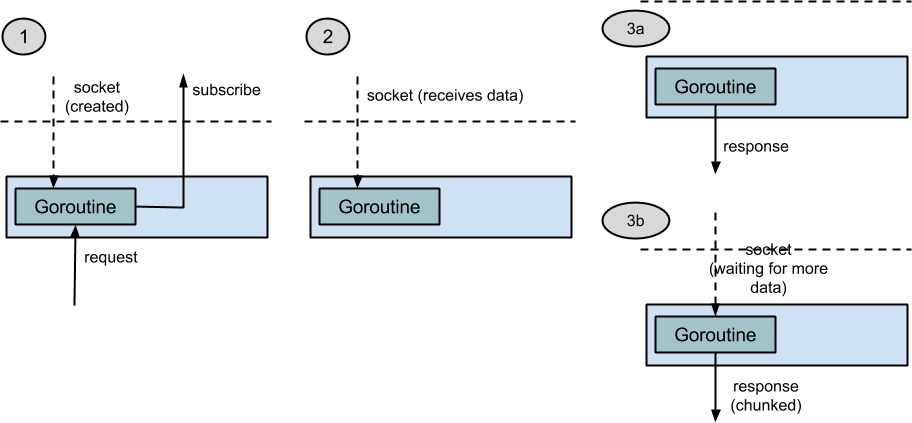
\includegraphics[scale=0.6]{implementation/images/api.png}
  \caption{The life cycle of a Request}\label{fig:api}
\end{figure}



% The cluster.
 
\chapter{TODO: The Cluster}
\label{sec:cluster}

% The hardware specifications.

\subsection{TODO: The Hardware}

Finalment això ho remato parlant del hardware (apartat 3.4). Sobre el hardware
comentaré les especificacions mínimes, les òptimes que ha de tenir el cluster
que executi aquest programa.


% Some benchmarks.

\section{Running this Platform}

\subsection{Local execution}

Asdad

\subsection{Remote execution}

asdad



% Section where I talk about what I needed to do in order to complete my
% thesis. Nothing too fancy...

\section{TODO: The Development of this Project}

% We first talk about the schedule.
 
\section{TODO: The Schedule}

En primera instància parlaré de la planificació del projecte: la planificació
original, com ha canviat, i finalment com ha sigut. Es tracta de explicar com
ha evolucionat tot plegat.


% Yeah, right, I had a budget ...

\section{Budget}

\subsection{Introduction}

In this delivery I am focusing on the budget and on the impact of my project.
First of all, I am going to focus on the budget. This includes doing some math
in the following topics: human resources, hardware and software.

Lastly, I will be explaining the impact that I expect that this project will
have. My only considerations for the impact will be the social impact and the
environmental impact.

\subsection{Budget}

In this section I will be describing the estimated costs that this project will
have. After specifying each of the costs, I will make up a total amount of
estimated costs. This will lead me to conclude the needed budget for this
project.

\subsection{Human resources}

What I want to do in this section is to describe all the costs related to
employing people to develop this project.

Luckily enough, it is just me in this project, so I just have to compute my own
salary. After doing some research, I have found that the average salary for a
Big data analyst is around 99,000 USD a year. This boils down to 51 USD per
hour. I did my scheduling based on weeks, instead of hours, and I think that I
will spend 20 hours in average per week. This means that in total, my salary
during the project will be:

\[
  20\ hours \cdot 16\ weeks \cdot 51\ USD = 16,320\ USD
\]


\subsection{Hardware}

Ideally in this section I would explain all the costs regarding the hardware.
However, I can't compute this because the only hardware that I will specify will
be the cluster which, in turn, is just a proposal. Other things like my laptop
won't be counted in this section They are not a cost for this project since I
use them for personal purposes too.

\subsection{Software}

In this section I will describe all the costs associated with software. In
short, this is my budget for software:

\[
  0\ \$
\]

All the software that I will be using for this project is free: both as in
``free beer'' as in ``free speech''. There are no fees for any license, I won't
be using any paid service, etc. Nothing.

\subsection{Total}

The main conclusion is that the only cost associated to this project is just my
salary. Therefore, my estimated costs are a total of \$16,320.

\subsection{Social impact}

This section is really important for this project. It is about the impact that
this platform will make to society. This is not a direct impact, but an
indirect one. The social impact of this platform comes in two ways:

\mylist
  \item The fact that a number of businesses will take advantage that this
platform exists.
  \item Indirectly, all the impact that all the services built on top of this
platform will produce.
\mylistend

This means that, ideally, the social impact of this platform can be huge.

\subsection{Environmental impact}

In the same way that this platform can bring a lot of goodness in the social
front, it certaintly comes with a cost. In my case the cost is an environmental
impact that cannot be understated.

In this project I will propose an ideal cluster that would be able to run the
software that I will design. The problem here is that maintaining a cluster
means the following:

\mylist
  \item Power supply.
  \item Maintaining a cooling system.
  \item The implied environmental costs of building the cluster.
\mylistend

All of these can be reduced by using the minimum amount of cluster time as
possible. This means to run the software in ``batches'' or with a very low
latency. However, this is not possible at all if the cluster has a lot of
requests, and that is to be expected.

Therefore, in the development of the cluster I will focus most of my efforts
into keeping the cluster as environmental friendly as possible.


% Additional sugar.
 
\subsection{TODO: Laws and Regulation}



% Social and environmental impact.

\chapter{Social and environmetal impact}

% About the environmental impact of the platform.

\section{TODO: Environmental impact}

In the same way that this platform can bring a lot of goodness in the social
front, it certaintly comes with a cost. In my case the cost is an environmental
impact that cannot be understated.

In this project I will propose an ideal cluster that would be able to run the
software that I will design. The problem here is that maintaining a cluster
means the following:

\mylist
  \item Power supply.
  \item Maintaining a cooling system.
  \item The implied environmental costs of building the cluster.
\mylistend

All of these can be reduced by using the minimum amount of cluster time as
possible. This means to run the software in ``batches'' or with a very low
latency. However, this is not possible at all if the cluster has a lot of
requests, and that is to be expected.

Therefore, in the development of the cluster I will focus most of my efforts
into keeping the cluster as environmental friendly as possible.



% About the social impact of the platform.
 
\section{TODO: Social impact}

This section is really important for this project. It is about the impact that
this platform will make to society. This is not a direct impact, but an
indirect one. The social impact of this platform comes in two ways:

\mylist
  \item The fact that a number of businesses will take advantage that this
platform exists.
  \item Indirectly, all the impact that all the services built on top of this
platform will produce.
\mylistend

This means that, ideally, the social impact of this platform can be huge.



% Additional sugar.
 
\subsection{TODO: Laws and Regulation}



% The conclusions of the whole thingie :D

\chapter{Conclusions}

We can debate a lot of things in Computer Science but, in the end, the only
thing that matters is if we have accomplished our goals. Looking back at the
very beginning of this memoir we can read the main goal for this project:

\begin{quote}
\centering
  ``The goal of this project is to build a base platform that is able to
generate rich information about a set of cities in real time.''
\end{quote}

So, have we accomplished this goal? I think so. Looking back we can see
that during this project I have accomplished the following milestones:

\begin{enumerate}
  \itemsep0em
  \item I have created a base platform that processes data in streaming. The
base platform can be extended to fetch data from other sources, it can be
extended to handle the data in a different way, etc. This platform is
extensible and rock solid.
  \item I have implemented a couple of services that prove that this platform
works. The two services that have been developed in this project are quite
minimalistic, but they both prove that the base platform is working and that a
lot of things can be achieved with this software.
  \item I have explored the limits of this platform, and I have explained them
along the way. This way I have been capable to determine the requirements of
the platform. Moreover, with these tests I have been able to give some hints on
how a cluster can be built to run this platform.
\end{enumerate}

Therefore, I believe that all the expectations for this project have been
met, and I could not feel more confident about it.


% TODO
\backmatter
\chapter{TODO: Bibliography}

Finalment ficaré l'apartat de bibliografia del projecte.

\end{document}
